\chapter{Introduction} \label{introduction}
\graphicspath{Figures/chapter1/}
\section{Graphs}
In this subsection, the main aspects of graph theory are briefly presented.
\subsection{Introduction}


% \subsubsection{Begginings and historical remarks}


% \subsubsection{Introduction}

In the real world, many problems can be described by a diagram connecting a set of points with
lines, joining pairs of these points, or even creating loops on a single point. A simple example
of that would be a set of points representing people with lines connecting acquintances, or
points representing atoms and lines representing chemical bonds, creating a representation of
a molecule as a graph attribute. In the examples above, the only information contained is whether
two points are associated, with the manner being disregarded. The concept of a graph consists of
a mathematical abstraction of the above. \cite{book:2008}


\begin{definition} \label{u_simple_graph} Mathematically, in its simplest form, a
  \textbf{graph} is an ordered pair\footnotemark{} $G=(V, E)$ of:
  \begin{itemize}
  \item \textbf{V}, a set of vertices (also known as nodes).
  \item $E \subseteq \{\{x, y\} | x,y \in V ~x \neq y \}$, which is the set of \textbf{edges}
    which consists of unordered pairs of vertices that connect two nodes.
  \end{itemize}
\footnotetext{An ordered pair $(a, b)$ is a pair of objects in which the order of
appearance or insertion is significant; the ordered pair $(a, b)$ is different than $(b,
a)$ unless $a=b$. An unordered pair is a set of the form ${a, b}$ is a set having two
elements with no relation between them and ${a, b} = {b, a}$.  }
\end{definition}

This type of object is called an \textbf{undirected simple graph} to avoid confusion
with other types.

\begin{definition}\label{graph_def}
  A \textit{graph} G is an ordered pair $(V(G), E(G))$ consisting of a set
$V(G)$ of \textit{vertices} (also called \textit{nodes} or \textit{points}) and a set
$E(G)$, disjoint from $V(G)$ which consists of \textit{edges} (also called \textit{links}
or \textit{lines}) together with an incidence function $\psi_G$ that associates with each
edge of G an unordered pair of not necesserily distinct vertices of G.  If $e$ is an edge
and $u$ and $v$ are vertices such that $\psi_G ={u, v}$ then $e$ is said to \textit{join}
$u$ and $v$, and the vertices $u$ and $v$ are called the \textit{ends} of $e$. We denote
the numbers of vertices and edges $G$ by $u(G)$ and $e(G)$ which two parameters are called
the \textit{order} and \textit{size} of G, respectively \cite{book:2008}.

  In short, we can define a \textbf{graph} as an ordered triple $G=(V, E, \phi_G)$
consisting of:
  \begin{itemize}
  \item $V$, a set of \textit{vertices}
  \item $E$, a set of \textit{edges}
  \item $\phi_G: E \rightarrow \{\{x, y\} | x, y \in V \; and \; x \neq y\}$ an
\textit{incidence function} mapping every edge to an unordered pair of vertices - an edge
associated with two distinct vertices. The incidence function is a function of the edges.
  \end{itemize} This type of object is called an \textit{undirected multigraph}, to avoid
confusion. Note, that the above definition of the \textit{incidence function} does not
allow for \textit{loops} (mappings of an edge on the same vertex).

A \textit{loop} is a an edge that allows a connection of a vertex to itself and a graph can
be defined to either allow or disallow the presence of loops. Some authors allow for loops
to exist on \textit{multigraphs} \cite{article:bollobas}, while other consider these kind
of graphs to exist in a different category, called \textit{pseudographs} \cite{book:Gary}.
Allowing loops requires modifying the incidence function so they can be supported. The new
incidence function can be written as:
\begin{equation}\label{eq:phi} \phi_G : E \rightarrow \{\{x, y \} | x,y \in V\} \end{equation}
The example presented below should better illustrate clarify the definition (of a pseudograph).
\begin{figure}[H]
  \begin{center}
  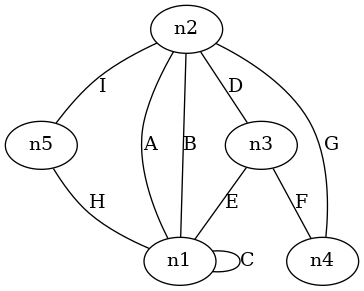
\includegraphics[scale=0.5]{Figures/chapter1/definition_ex_1.png}
\end{center}
  \caption{An undirected pseudograph with labeled nodes and
edges.}\label{fig:SimplePseudograph}

\end{figure}
\begin{example}

  \

For the graph presented in  \fref{fig:SimplePseudograph}  the following
can be assumed:
\begin{align*}
    &G = (V(G), E(G))
    &\intertext{and} 
    &V(G) = \{n_1, n_2, n_3, n_4, n_5\} \\
    &E(G) = \{A, B, C, D, E, F, G, H, I\} 
    &\intertext{and the incidence function is defined as:}
    &\psi_G(A) = n_1n_2,\quad \psi_G(B) = n_1n_2, \quad \psi_G(C) =
      n_1n_1, \quad \psi_G(D) = n_2n_3,\\
    &\psi_G(E) = n_1n_3, \quad \psi_G(F) = n_3n_4, \quad \psi_G(G) = n_2n_4,
      \quad \psi_G(H)= n_1n_5, \\
    &\psi_G(I) = n_2n_5
\end{align*}
\end{example}
  
It should now be clear that with the newer definition of $\phi_G$, self loops are now possible.
Additionaly, even though this was not prohibited by the previous definition, it is worth
noting that a node can be connected to another with multiple edges (or multiedges), or that it can have zero
connections to other nodes. Generally, $V$ is assumed to be a non-empty set, but $E$ can be
empty.

It is now possible to define some characteristic attributes of graphs:
\begin{itemize}
\item $|V|$: the \textbf{order} of a graph is the number of its vertices.
\item $|E|$: the \textbf{size} of a graph is the number of its edges.
\item The \textbf{degree} (or \textbf{valency}) of a single node is the number of
  edges connected to it. The \textbf{degree} of a graph is the maximum number of
  edges connected to a single vertex that belongs to it.
\item The edges of create a \textit{homogenous relation}\footnotemark{} $\sim$ on the vertices
  of the graph that is called \textbf{adjacency relation}; for each edge \textit{$(x, y)$}, its
  endpoints \textit{x, y} are said to be \textbf{adjacent} to each other, denoted by $x \sim y$.
  This property will be particulary useful when the adjacency matrix is defined in the following
  section.
\end{itemize}

\footnotetext{A \textbf{homogenous relation} (or \textbf{endorelation}) over a set \textit{X}
  is a set of assignments (binary relations) over \textit{X} and itself; i.e. it is a subset of
  the cartesian product $X\times X$
}

It can be inferred from the above definitions and attributes that for an undirected
graph of order \textit{n}, the maximum \textit{degree} of a node is $n~-~1$ and
and maximum \textit{size} of a graph is $n(n~-~1)/2$.

\end{definition}

In this section only \textit{undirected} graphs were considered, which are graphs
with edges with no orientation. A whole other class of graph objects with edges which
have orientation exists, called \textit{directed graphs}. These kind of graphs objects
are out of scope for this thesis and will not be presented.


\subsection{Adjacency Matrix}
\begin{definition}
  The \textit{adjacency matrix} is the fundamental mathematical representation of a graph.
  It is a square matrix, the elements of which represent which pair of nodes are
  \textit{adjacent} or not. Thus, the adjacency matrix \textbf{A} of a graph of order $n$
  is the $n\times n$ matrix with elements $A_{ij}$ such that:
  \begin{equation}
    \label{eq:adj_mat}
    A_{ij} = \begin{cases} 1 &\text{if there exists at least one edge connecting $i$ and $j$} \\
               0 &\text{if there no edges connecting those edges directly.}

             \end{cases}
\end{equation}
\end{definition}


\begin{figure}
     \begin{subfigure}[t]{0.4\textwidth}
         \centering
         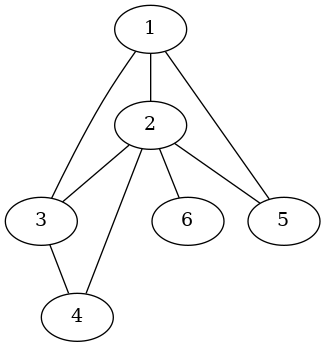
\includegraphics[width=\textwidth]{Figures/chapter1/simple_graph_adj.png}
         \caption{Multigraph with no loops and multiple edges.}
         \label{fig:simple_adj_demo}
     \end{subfigure}
     \hfill
     \begin{subfigure}[t]{0.4\textwidth}
         \centering
         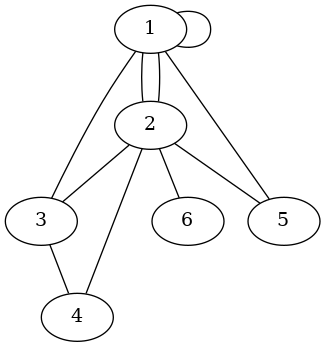
\includegraphics[width=\textwidth]{Figures/chapter1/complex_graph_adj.png}
         \caption{Mutligraph with loops and multiple edges.}
         \label{fig:compl_adj_demo}
     \end{subfigure}
        \caption{Two undirected multigraphs.}
        \label{fig:two multigraphs}
\end{figure}

Considering the simple undirected graph of \fref{fig:simple_adj_demo} we can construct
the following adjacency matrix:
\begin{table}[H]
  
  \begin{equation*}
    A = 
    \begin{pmatrix}
      0 & 1 & 1 & 0 & 1 & 0 \\
      1 & 0 & 1 & 1 & 1 & 1 \\
      1 & 1 & 0 & 1 & 0 & 0 \\
      0 & 1 & 1 & 0 & 0 & 0 \\
      1 & 1 & 0 & 0 & 0 & 0 \\
      0 & 1 & 0 & 0 & 0 & 0 
    \end{pmatrix}
  \end{equation*}
  \caption{Adjacency matrix for \fref{fig:simple_adj_demo}}
\end{table}

For this simple network, which has no loops and only one edge connect two nodes,
the diagonal matrix elements are always zero and the matrix is symmetric, as for
each edge connecting $i$ and $j$ there is a representation for the $j$ to $i$ connection
as well.

In a more complex case, such as the one presented in \fref{fig:compl_adj_demo} where loops
and multiedges are present an adjacency matrix can still be constructed. In this case,
a multiedge is represented by setting the value of the corresponding $A_{ij}$ value equal
to the multiplicity of the edge. In this case, $A_{12} = A_{21} = 2$.

For loops, the most common representation in the case of undirected
graphs is to still set the value of the $A_{ii}$ element equal to $2$
(i.e. $A_{11} = 2$ in the example presented).  Essentially, an edge of
a loop has two ends that connect to the same node, thus the result
\cite[p.~68]{book:algebraic}. Additionaly, defining the matrix in such
manner, allows for better computations and is consistent with the
definition of the representation of an edge connecting two nodes of an
undirected graph \cite[p.~108]{book:Newman}. 

Thus, the adjacency matrix for the graph of \fref{fig:compl_adj_demo} is

\begin{table}[H]
  \begin{equation*}
    A = 
   \begin{pmatrix}
      2 & 2 & 1 & 0 & 1 & 0 \\
      2 & 0 & 1 & 1 & 1 & 1 \\
      1 & 1 & 0 & 1 & 0 & 0 \\
      0 & 1 & 1 & 0 & 0 & 0 \\
      1 & 1 & 0 & 0 & 0 & 0 \\
      0 & 1 & 0 & 0 & 0 & 0 
    \end{pmatrix}
  \end{equation*}
  \caption{Adjacency matrix for  \fref{fig:compl_adj_demo}}
\end{table}
